% siminos/CLE/CLE.tex
% $Author$ $Date$

                            \newif\ifdraft \newif\ifpaper
  \drafttrue\paperfalse      % draft version, commented
%   \draftfalse\paperfalse     % final version, hyperlinks
% \draftfalse\papertrue      % final version, no hyperlinks, for printing
%%%%%%%%%%%%%%%%%%%%%%%%%%%%%%%%%%%%%%%%%%%%%%%%%%%%%%%%

% Predrag reorganized siminos/CLE/          2009-10-09
% Vaggelis created siminos/CLE/CLE.tex      2009-09-21
% Vaggelis created siminos/CLE              2009-02-05

\ifdraft
\documentclass[preprint,number,sort&compress]{elsarticle}
\else
\documentclass[final,number]{elsarticle}
\fi

\usepackage{amsmath,amsfonts,amssymb,amsbsy,amscd}
\usepackage{ifthen}
\usepackage{graphicx}
\usepackage[dvips]{color}
\usepackage[dvips,colorlinks]{hyperref}
\graphicspath{{../figs/}{../Fig/}}  %% directories with graphics files
\input ../inputs/def        % TEMPORARY
\input inputs/defsCLE.tex   % eventualy merge used commanDs into inputs/defsCLE.tex

% Use the next command to get Bibliography header appear. The problem is a conflict
% between elsarticle and amsref over \bibsection command.
 \renewcommand\bibname{References}
 \newcommand\bibsection{%
   \section*{\bibname\markright{\MakeUppercase{\bibname}}}}

\begin{document}
\journal{Physica D}
\begin{frontmatter}

\ifdraft
			\title{
Oh, you poor Yooropions, befuddled by the subtleties of English articles.
			}
\else
			\title{
Continuous symmetry reduction and return maps for higher-dimensional flows
			}
% Continuous symmetry reduction and return maps for high dimensional flows
% Continuous symmetry reduced return maps for high dimensional flows
% Returm maps of high dimensional flows with continuous symmetry:
%                                           I. Symmetry reduction
% Towards continuous symmetry reduction in high dimensional flows
\fi

\author{Evangelos Siminos}
\ead{siminos@gatech.edu}
\author{Predrag Cvitanovi\'c}
\address{Center for Nonlinear Science,
School of Physics, Georgia Institute of Technology,
Atlanta, GA 30332-0430}
%\homepage[]{Your web page}
%\thanks{}
%\altaffiliation{}

\date{\today}

        \begin{abstract}
We present two continuous symmetry reduction methods for
reducing high-dimensional dissipative flows to local return
maps. In the Hilbert polynomial basis approach the equivariant
dynamics is rewritten in terms of invariant coordinates. In the
`method of moving frames' or `method of slices' the state space
is `sliced' locally in such a way that each group orbit of
symmetry-equivalent points is represented by a single point. In
either approach, numerical computations can be performed in the
original state-space representation, and the solutions are then
projected onto the symmetry-reduced state space. The two methods
are illustrated by reduction of the complex Lorenz system, a
5-dimensional dissipative flow with rotational symmetry. While
the Hilbert polynomial basis approach appears to be infeasible for
high-dimensional flows, symmetry reduction by the `method of
moving frames' offers hope.
        \end{abstract}

\begin{keyword}
continuous symmetry reduction,
relative equilibria,
relative periodic orbits,
return maps,
slices,
moving frames,
Hilbert polynomial bases
\PACS 05.45.-a \sep 47.27.ed \sep 42.65.Sf
% 05.45.-a 	Nonlinear dynamics and chaos
% 05.45.Jn 	High-dimensional chaos
% 47.10.Fg 	Dynamical systems methods (in Fluid Mechanics)
% 47.27.ed 	Dynamical systems approaches (turbulent flows)
% 47.52.+j 	Chaos in fluid dynamics
% 42.65.Sf 	Dynamics of nonlinear optical systems; optical instabilities,
% 		optical chaos and complexity, and optical spatio-temporal dynamics
\end{keyword}
\end{frontmatter}

\section{\label{s:intro} Introduction}
    % former siminos/CLE/intro.tex

In his seminal paper, E. Lorenz\rf{lorenz} reduced the
continuous time and discrete spatial symmetries of the
3-dimensional Lorenz equations, resulting in a 1-dimensional
return map that yields deep insights\rf{tucker1-2} into the
nature of chaos in this flow. For strongly contracting,
low-dimensional flows, Gilmore, Lefranc and
Letellier\rf{gilmore2003,GL-Gil07b} systematized construction
of such discrete time return maps, through use of topological
templates, Poincar\'e sections (to reduce the continuous time
invariance) and invariant polynomial bases (to reduce the
spatial symmetries). They showed that in presence of spatial
symmetries one has to  `quotient' the symmetry and replace
the dynamics by a physically equivalent reduced,
desymmetrized flow, in which each family of symmetry-related
states is replaced by a single representative. This approach
leads to symbolic dynamics and labeling of all \po s up to a
given topological period. Periodic orbit theory can then
yield accurate estimates of long-time dynamical averages,
such as Lyapunov exponents and escape rates\rf{DasBuch}.
    \PC{
    remove PC\{\} and PCedit\{\}, \etc,
    after you have accepted/edited them
    }

In a series of papers Cvitanovi\'{c}, Putkaradze,
Christiansen and Lan%
\rf{Christiansen97,chfield,LanThesis,CvitLanCrete02,lanVar1,lanCvit07}
showed that effectively low-dimensional return maps can be
constructed for high-dimensional (formally infinite
dimensional)  flows described by dissipative partial
differential equations (PDEs) such as the \KSe\ (KS). Such
flows have state-space topology vastly more complicated than
the Lorenz flow, and collections of local Poincar\'e sections
together with maps from a section to a section are required
to capture all of the important asymptotic dynamics. These KS
studies were facilitated by a restriction to the
flow-invariant subspace of odd solutions, but at a price:
elimination of the translational symmetry of the KS system
and with it physically important phenomena, such as traveling
waves. Traveling (or `relative') unstable coherent solutions
are ubiquitous and play a key role in organization of
turbulent hydrodynamic flows, as revealed both by
simulations\rf{KawKida01,FE03,WK04,Visw07b,GHCW07} and
experimentation\rf{science04}.
    \ES{update references}
For KS\rf{SCD07,SiminosThesis}, and even for a relatively
low-dimensional flow such as the
\cLe\rf{GibMcCLE82,FowlerCLE82} used as an example here, with
the simplest possible continuous (rotational) spatial
symmetry, the symmetry-induced drifts obscure the underlying
hyperbolic dynamics.

The question that we address here is how one can construct
suitable return maps for arbitrarily high-dimensional but
strongly dissipative flows in presence of continuous
symmetries. Our exposition is based in part on
\refrefs{SiminosThesis,DasBuch,Wilczak09}. The reader is
referred to the monographs of Golubitsky and
Stewart\rf{golubitsky2002sp}, Hoyle\rf{hoyll06},
Olver\rf{OlverInv}, Bredon\rf{Bredon72}, and
Krupa\rf{Krupa90} for more depth and rigor than would be wise
to wade into here.

In \refsect{s:symDyn} we review the basic notions of symmetry
in dynamics. \refSect{s:introCLE} introduces the \SOn{2}\
equivariant \cLe\ (CLE), a 5-dimensional set of ODEs that we
use throughout the paper to illustrate the strengths and
drawbacks of different symmetry reduction methods. In
\refsect{s:symSol} we describe important classes of solutions
and their symmetries: \eqva, \reqva, \po\ and \rpo s, and use
them motivate the need for symmetry reduction.

In \refsect{s:Hilbert} we briefly review one of the standard tools
by which spatial symmetry reduction can be achieved:
projection to a Hilbert basis.
In \refsect{sec:mf} we review the {\mframes}, a direct and
efficient method that goes back to Cartan for computing
symmetry-invariant bases, and in \refsect{sec:CLeMovFr} we
illustrate this method in application to the \cLe. The method
maps all solutions to a `slice,' a submanifold  of state
space that plays a role for group orbits akin to the role
Poincar\'e sections play in reducing continuous time
invariance. In contrast to the Hilbert basis approach, slices
are local, and more than one slice might be needed to
capture the flow globally. In \refsect{s:laserMFnum} we show
that a single local slice can suffice for the purpose of
reducing the \cLe\ flow to a return map.
    \ES{Create subsection if that part stays in the paper.
    {\bf PC} dropped:
    We discuss some remedies to the
    situation in \refsect{sec:mf}.}
In \refsect{sec:MovFrameODE} we recast the {\mframes}
into the equivalent, differential \mslices, with
time integration
restricted to a slice fixed by a given \statesp\ point.
As the slice is local, both methods suffer from the same
restrictions, with generic trajectories within a slice bound to encounter
singularities.

\PublicPrivate{}{
In \ref{s:StabReq} we derive an expression for the stability
of \reqva\ (traveling waves) in \reducedsp\
that can be applied without an explicit
calculation of the reduced system.
    \PC{unless you clean up \ref{s:StabReq} now, it will have to
        be omitted.}
    } %end \PublicPrivate{}{


\section{\label{s:symDyn} Symmetries of dynamical systems}
% former siminos/CLE/symDyn.tex

Consider a system of \ode s of the form
\beq
	\dot{\ssp} = \vf(\ssp)
	\label{eq:difeq}
\eeq
with $\vf$ a smooth vector field and $\ssp\in\pS\subset\Rls{d}$.
Here are interested in the role continuous symmetries
play in dynamics.
While the key concepts and methods we develop here are well
illustrated by the 1-parameter Lie \SOn{2} group, they are in
principle applicable to any compact Lie group, and the
generalization to translational and rotational symmetries of
PDEs such as \KS\ and \pCf\ is immediate.

A linear action $\LieEl$ is a symmetry of
\refeq{eq:difeq} if
\beq
	\vf(\LieEl \ssp) =\LieEl \, \vf(\ssp)
	\label{eq:equiv}
\eeq
for all $\ssp\in\Rls{d}$. One  says that $\vf$ \emph{commutes}
with $\LieEl$ or that $\vf$ is $\LieEl$-\emph{equivariant}.
When $\vf$ commutes with the set of group elements
$\LieEl\in\Group$, the vector field $\vf$ is said to be
$\Group$-equivariant. The group $\Group$ is said to be a {\em
symmetry} of dynamics if for every solution $\ssp(\tau)=
\flow{\tau}{\ssp}$, $\LieEl \, \ssp(\tau)$ is also a solution. The finite
time flow $\flow{\tau}{\LieEl \ssp}$ through $\LieEl \ssp$ then
satisfies the equivariance condition
\beq\label{eq:equivFinite}
\flow{\tau}{\LieEl \ssp}=\LieEl\flow{\tau}{\ssp}
\,.
\eeq
In physics literature the term $invariant$ is most commonly
used; for example, in Hamiltonian systems a symmetry is
manifested as invariance of the Hamiltonian under the
symmetry group action.

An element of a compact Lie group
continuously connected to identity can be written as
\beq
\LieEl(\gSpace)=e^{\gSpace \cdot \Lg }
	\,,\qquad
\gSpace \cdot \Lg  = \sum \gSpace_a \Lg_a,\; a=1,2, \cdots, N
\,,
\ee{FiniteRot}
where
$\gSpace \cdot \Lg$
is a {\em Lie algebra} element,  and $\gSpace_a$ are the parameters
of the transformation. Repeated indices are summed throughout this
chapter, and the dot product refers to a sum over
Lie algebra generators. The Euclidian product of two vectors
$x,y$ is indicated by $x$-transpose times $y$, \ie,
$x^T y = \sum_i^d x_i y_i$.
Finite transformations $ \exp(\gSpace \cdot {\Lg}) $ are
generated by sequences of infinitesimal steps of form
\beq
\LieEl(\delta\gSpace) \simeq 1 + \delta \gSpace \cdot \Lg
% \LieEl{}_i{}^j \simeq \delta_i^j +  \delta \gSpace_a \, (\Lg_a)_i^j
    \,,\quad
\delta\gSpace \in \reals^N
    \,,\quad
|\delta \gSpace| \ll 1
    \, ,
\ee{intsmLieTransf}
where $\Lg_a$, the {\em generators} of infinitesimal
transformations, are a set of $N$ linearly independent
$[d\!\times\!d]$ anti-hermitian matrices, $(\Lg_a)^\dagger =
- \Lg_a$, acting linearly on the $d$-dim\-ens\-ion\-al \statesp\
$\pS$.
The flow
at the \statesp\ point $\ssp$ induced by the action of the group
is given by the set of $N$ tangent fields
\beq
\groupTan_a(\ssp)_{i}= (\Lg_a){}_{ij} \ssp_j
\,.
\ee{GroupTangField}

For an infinitesimal transformation \refeq{intsmLieTransf}
the $\Group$-equivariance condition \refeq{eq:equiv}
becomes
\[
\vel(\ssp)
      \simeq
  (1-\gSpace \cdot \Lg) \, \vel(\ssp+\gSpace \cdot \Lg \, \ssp)
       = \vel(\ssp)- \gSpace \cdot \Lg \, \vel(\ssp)
             + \frac{d\vel}{d\ssp} \,\gSpace \cdot \Lg \, \ssp
\,.
\]
Denote
the group flow tangent field at \ssp\ by
$\groupTan_a(\ssp)_{i}= (\Lg_a){}_{ij} \ssp_j$. Thus the
infinitesimal, Lie algebra $\Group$-equivariance condition is
\beq
  \groupTan_a(\vel)  - \Mvar(\ssp) \, \groupTan_a(\ssp) =0
  \,,
\ee{inftmInv}
where $\Mvar = {\pde \vel}/{\pde \ssp}$ is the \stabmat.
The left-hand side,
\beq
{\cal L}_{\groupTan_a} \vel =
\left.\left(
  \Lg_a - \frac{\partial}{\partial y}(\Lg_a \ssp)
 \right) \vel(y)\right|_{y=\ssp}
 \,,
\ee{LieDeriv}
is known as
the {\em Lie derivative} of the dynamical flow
field $\vel$ along the direction of the infinitesimal
group-rotation induced flow $\groupTan_a(\ssp)= \Lg_a \ssp$.
The equivariance condition \refeq{inftmInv} states that the two
flows, one induced by the dynamical vector field $\vel$, and
the other by the group tangent field $\groupTan$, commute if
their Lie derivatives (or the `Lie brackets ' or `Poisson
brackets') vanish.

Any representation of a compact Lie group $\Group$ is fully
reducible, and invariant tensors constructed by contractions
of $\Lg_a$ are useful for identifying irreducible
representations. The simplest such invariant is
\beq
\Lg^T \cdot \Lg = \sum_\alpha C_2^{(\alpha)} \, \id^{(\alpha)}
\,,
\ee{QuadCasimir}
where $C_2^{(\alpha)}$ is the quadratic Casimir for
irreducible representation labeled $\alpha$, and
$\id^{(\alpha)}$ is the identity on the $\alpha$-irreducible
subspace, 0 elsewhere. The dot product of two tangent fields
is thus a sum weighted by Casimirs,
\beq
\groupTan(\ssp)^T  \cdot \groupTan(\ssp')
   = \sum_\alpha C_2^{(\alpha)} \ssp_i\, \delta_{ij}^{(\alpha)} \ssp'_j
\,.
\ee{dotProd}


\subsection{\label{s:introCLE} An example: \CLe}
% former siminos/CLE/introCLE.tex
% from siminos/thesis/lasersSym.tex and
% ChaosBook chapter continuous.tex {Relativity for cyclists} 18 Jan 2010

Consider a complex generalization of Lorenz equations,
\bea
 \dot{x} &=& -\sigma x+ \sigma y \,,\qquad
 \dot{y} \,=\, (\rLor-z)x-a y \continue
 \dot{z} &=& (x y^*+x^*y)/2 -b z\,,
 \label{eq:CLe}
\eea
where $x,y$ are complex variables, $z$ is real, while the
parameters $\sigma,\,b$ are real and $\rLor=\RerCLor+i
\ImrCLor$, $a=1-i e$ are complex. Recast in real variables,
this is a set of five coupled ODEs
\bea
	\dot{x}_1 &=& -\sigma x_1 + \sigma y_1
            \,,\quad
	\dot{x}_2 \,=\, -\sigma x_2 + \sigma y_2\continue
	\dot{y}_1 &=& (\RerCLor-z) x_1 - \ImrCLor x_2 -y_1-e y_2 \continue
	\dot{y}_2 &=& \ImrCLor x_1 + (\RerCLor-z) x_2 + e y_1- y_2\continue
	\dot{z} \; &=& -b z + x_1 y_1 + x_2 y_2
    \,.
\label{eq:CLeR}
\eea
In all numerical examples that follow, the parameters will be
set to $\RerCLor=28,\, \ImrCLor=0,\, b=8/3,\, \sigma=10,\, e=
1/10$, unless explicitly stated otherwise.
%
%%%%%%%%%%%%%%%%%%%%%%%%%%%%%%%%%%%%%%%%%%%%%%%%%%%%%%%%%%%%
% plotted with vaggelis/testing/flows/CLEfinalTmp.nb
% Used snippet of code from  >> >> /CLEdefense.nb
% To get same eps bounding box for both when merging text and
% graphics used bounding box from plCLE.eps figure
% with all trajectories combined.
\begin{figure}[ht]
\begin{center}
  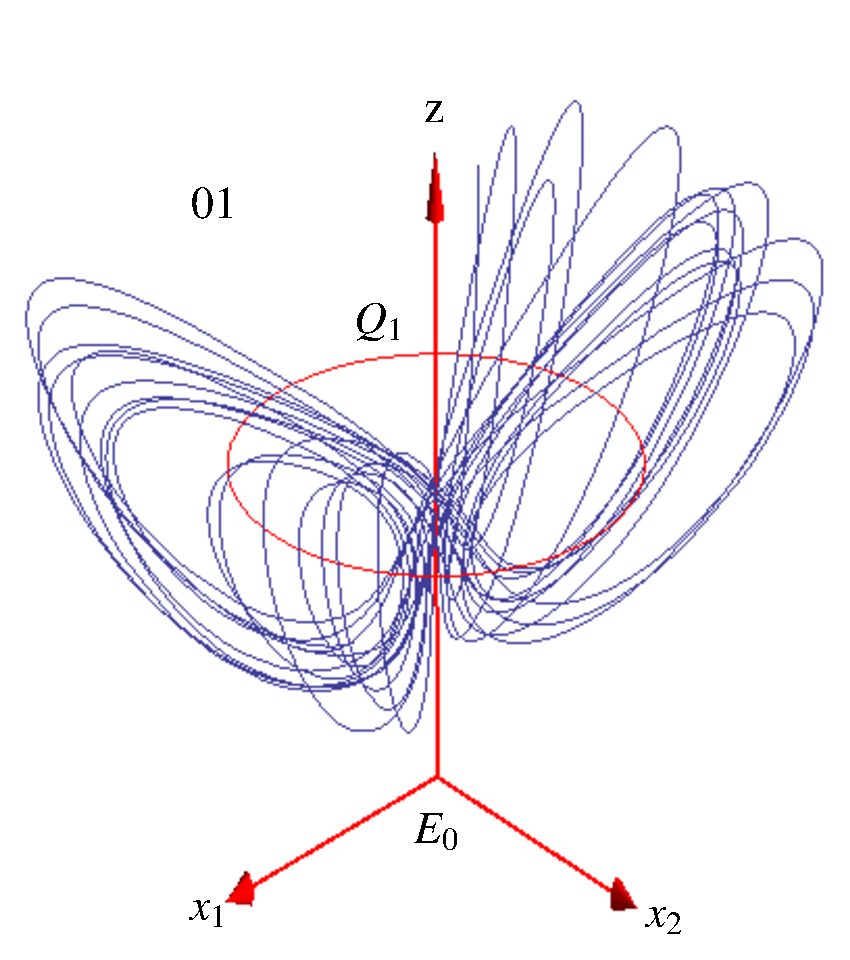
\includegraphics[width=0.40\textwidth, clip=true]{CLEchaotic}
  \includegraphics[width=0.40\textwidth, clip=true]{CLEcompact}
\end{center}
\caption{
\Statesp\ portrait of \cLf. Plotted are a generic chaotic trajectory (blue),
\eqv\
\EQV{0}, a representative of its unstable manifold (green),
\reqv\ \REQV{}{1} (red), its unstable manifold (brown), and
three repeats of the \cycle{01} \rpo.
}
\label{fig:CLE}
\end{figure}
%%%%%%%%%%%%%%%%%%%%%%%%%%%%%%%%%%%%%%%%%%%%%%%%%%%%%%%%%%%%
%
Why worry about continuous symmetries? The visualization
in \reffig{fig:CLE} of typical long-time dynamics of \cLf\ suffices
to illustrate the effect a continuous symmetry has on
dynamics. A generic trajectory slowly `drifts' along the
direction of continuous symmetry while tracing a
Lorenz-butterfly like attractor. It is a mess.

The \CLe\ are a dynamical system with a continuous
(but no discrete) symmetry, equivariant under the one-parameter
rotation group $\Un{1}\cong\SOn{2}$ acting by
\beq\label{eq:SO2cle}
	(x,\,y,\,z)\mapsto (
    e^{i\theta}x,\,e^{i\theta}y,\,z)\,,\ \theta\in[0,2\pi]
\,.
\eeq
Alternatively, substituting the Lie algebra generator
\beq
 \Lg \,=\,   \left(\barr{ccccc}
    0  & -1 & 0  &  0 & 0  \\
    1  &  0 & 0  &  0 & 0 \\
    0  &  0 & 0  & -1 & 0  \\
    0  &  0 & 1  &  0 & 0 \\
    0  &  0 & 0  &  0 & 0
    \earr\right)
\ee{CLfLieGen}
acting on a 5-dim\-ens\-ion\-al space \refeq{eq:CLeR} into
\refeq{FiniteRot} yields the  $\Rls{5}$ representation of a
finite angle action \refeq{eq:SO2cle} of $\SOn{2}$
\beq
\LieEl(\gSpace) \,=\,  \left(\barr{ccccc}
  \cos \gSpace  & -\sin \gSpace  & 0 & 0 & 0 \\
  \sin \gSpace  &  \cos \gSpace  & 0 & 0 & 0 \\
 0 & 0 &  \cos \gSpace & -\sin \gSpace   & 0 \\
 0 & 0 &  \sin \gSpace &  \cos \gSpace   & 0 \\
 0 & 0 & 0             & 0               & 1
    \earr\right)
\,.
\ee{CLfRots}
We see that the linear action of \SOn{2}\
on the \statesp\ of the \cLe\
decomposes into the $m\!=\!0$ \Group-invariant
subspace ($z$-axis) and  the $m=1$ subspace of multiplicity 2.

The generator $\Lg$ is anti-hermitian,
$\Lg^\dagger = - \Lg$, and the group is compact, its
elements parametrized by $\gSpace \mbox{ mod } 2\pi$. Locally, at
$\ssp \in \pS$, the infinitesimal action of the group is
given by the group tangent field $\groupTan(\ssp) = \Lg \ssp
= (-x_2,x_1,-y_2,y_1,0)$. In other words, the flow induced by
the group action is normal to the radial direction in the
$(x_1,x_2)$ and $(y_1,y_2)$ planes, while the $z$-axis is left
invariant.

The equivariance of the \cLf\ under $\SOn{2}$ rotations
\refeq{CLfRots} can be verified
by substituting the Lie algebra generator
\refeq{CLfLieGen} and the \stabmat\ for \cLf\ \refeq{eq:CLeR},
  \beq
\Mvar =
  \left(\barr{ccccc}
    -\sigma    	& 0 		& \sigma & 0    &  0 \\
	0 	& -\sigma       & 0      & \sigma   &  0 \\
	\RerCLor-z  &     -\ImrCLor      & -1     & -e & -x_1 \\
	\ImrCLor     & \RerCLor-z       	& e  	& -1       & -x_2 \\
	y_1     & y_2           & x_1    & x_2      & -b
    \earr\right)
\,,
  \ee{CLeStabMat}
into the equivariance condition \refeq{inftmInv}.
For the parameter values \refeq{eq:CLeR} the flow
is strongly volume contracting,
\beq
\pde_i \pVeloc_i
 = \sum_{i=1}^{5} \Lyap_i(\ssp,t)
= -b -2(\sigma + 1)
= -24 - 2/3
    \,,
\ee{trA-ZM}

The \CLe\ \refeq{eq:CLe} were introduced by
Gibbon and McGuinness\rf{GibMcCLE82,FowlerCLE82} as a
low-dim\-ens\-ion\-al model of baroclinic instability in the
atmosphere. Ning and Haken\rf{NingHakenCLE90} have shown that
equations isomorphic to the \cLe\ also appear as a truncation of
Maxwell-Bloch equations describing a single mode, detuned,
ring laser. They set $e+\ImrCLor=0$ (see \refeq{eq:omegaCLE})
so that \SOn{2}-orbits of detuned \eqva\
exist\rf{FowlerCLE82}. Zeghlache and Mandel\rf{ZeMa85} also
use equations isomorphic to \cLe\ with $e+\ImrCLor=0$ in
their studies of detuned ring lasers. This choice is
`degenerate' in the sense that it leads to non-generic
bifurcations. As the existence of \reqva\ in systems with \SOn{2}
symmetry is the generic situation, we follow Bakasov and
Abraham\rf{BakasovAbraham93} who set $\ImrCLor=0$ and $e \neq
0$.

Here, however, we are not interested in the physical
applications of these equations; rather, we study them as a
simple example of a dynamical system with continuous (but no
discrete) symmetries, with a view of testing methods of
reducing the dynamics to a lower-dimensional \reducedsp.
    \PC{looks like one should also read \refref{Abraham95}; they
    report on various return maps}
We investigate
various ways of `quotienting' its \SOn{2} symmetry, and
reducing the dynamics to a 4-dim\-ens\-ion\-al \reducedsp. As
we shall show, the dynamics has a nice {\stretchf}
action, but that is totally masked by the continuous symmetry
drifts. We shall not rest until we attain the simplicity of
\reffig{fig:CLEmfReqb1}, and the bliss of 1-dim\-ens\-ion\-al
return map of \reffig{fig:CLEipRM}.


\section{\label{s:symSol} Symmetries of solutions}
% former siminos/CLE/symSol.tex

In order to explore the implications of equivariance \JFGedit{on}
solutions of dynamical equations,  we start by examining the
way a compact Lie group acts on \JFGedit{a} \statesp\ \pS. The
\emph{group orbit} or \emph{$\Group$-orbit} of the point
$\ssp \in \pS$ is the set
\beq
    \pS_\ssp = \{\LieEl\,\ssp \mid \LieEl \in {\Group}\}
\ee{GroupOrb}
of all \statesp\ points into which $\ssp$ is mapped under the
action of $\Group$.
The \emph{symmetry} $\stab{\ssp}$ (\emph{isotropy} or
\emph{stabilizer} group) of a \statesp\ point $\ssp$ is the
largest subgroup of $\Group$
\beq
\stab{\ssp} =\{\LieEl \in \Group: \LieEl \ssp = \ssp \}
\ee{def:isotr}
that leaves $\ssp$ fixed.
The \emph{symmetry} $\stab{X}$ of a set $\pS_X \in \pS$ is
the largest subgroup  of $\Group$ that leaves $\pS_X$
invariant as a set:
\[
	\stab{X}= \{\LieEl: \LieEl \, \pS_X = \pS_X\}
\,.
\]
If $\stab{p}$ is a symmetry, intrinsic properties of a
solution $\pS_p$ (such as \eqv\ or a cycle stability
eigenvalues, period, Floquet multipliers) evaluated anywhere
along its $\stab{p}$-orbit are the same. A symmetry thus
reduces the number of inequivalent solutions. So we also need
to describe the symmetry of a \emph{solution}, as opposed to
\refeq{eq:equivFinite}, the symmetry of the \emph{system}.

The \emph{\fixedsp} $\Fix{\Subgroup}$ of a subgroup
$\Subgroup\subset\Group$ is the subspace of $\pS$ containing
all fixed points of $\Subgroup$:
\[
	\Fix{\Subgroup}=
      \{\ssp\in\pS,\,\LieEl\in\Subgroup \,|\,
        \LieEl \ssp = \ssp \}
\,.
\]
The physical importance of \fixedsp s lies in the fact that
they are invariant under $\Group$-equivariant
dynamics\rf{golubitsky2002sp},
\[
 f^\tau\left(\Fix{\Subgroup}\right)\subseteq \Fix{\Subgroup}
\]
and thus \emph{flow invariant} for all times $\tau$.
Therefore if $\ssp(\tau)$ is a solution of an equivariant ODE,
then its symmetry $\stab{\ssp(\tau)}=\stab{\ssp(0)}$ is
preserved for all times.

%
%%%%%%%%%%%%%%%%%%%%%%%%%%%%%%%%%%%%%%%%%%%%%%%%%%%%%%%%%%%%%%%%
% hand-drawn in dasbuch/book/FigSrc/xfig/rpo.fig
\begin{figure}[ht]
 (\textit{a})\includegraphics[width=0.40\textwidth,clip=true]{reqv}
~(\textit{b})\includegraphics[width=0.40\textwidth,clip=true]{rpo}
\caption{
(a) A {\em \reqv\ orbit} starts out at some point $\ssp(0)$,
with the dynamical flow field $\vel(\ssp) = \velRel \cdot
\groupTan(\ssp)$ pointing along the group tangent space. For
the $\SOn{2}$ symmetry depicted here, the flow traces out the
group orbit of $\ssp(0)$ in time $\period{}=2\pi/\velRel$.
An
{\em \eqv} lives either in the $\Fix{\Group}$ subspace
($x_3$ axis in this sketch), or on a group orbit as the one
depicted here, but with zero angular velocity $\velRel$. In
that case the circle (in general, $N$-torus) depicts a
continuous family of fixed \eqva, related only by the group
action.
(b) A {\em \rpo} starts out at $\ssp(0)$ with the dynamical $\vel$ and
group tangent $\groupTan$ flows pointing in different
directions, and returns to the group orbit of $\ssp(0)$ after
time $\period{p}$ at $\ssp(\period{p})=\LieEl_p \ssp (0)$, a
rotation of the initial point by $\LieEl_p$.
}
\label{f:rpo}
\end{figure}
%%%%%%%%%%%%%%%%%%%%%%%%%%%%%%%%%%%%%%%%%%%%%%%%%%%%%%%%%%%

In contrast to \emph{\eqv} solutions that satisfy
$f^\tau(\ssp)  =  \ssp$, \emph{\reqva} (or \emph{traveling
waves}) satisfy $f^\tau(\ssp) = \LieEl( \tau) \, \ssp$ for
any $\tau$. In a co-moving frame moving along the group orbit
with velocity $\vel(\ssp) = \velRel \cdot \groupTan(\ssp)$,
the \reqv\ appears as an \eqv. Here $\groupTan$ is the
group tangent field \refeq{GroupTangField}.

A {\em \rpo} is an orbit $\pS_p$ for which the initial point
exactly recurs
\beq
\ssp_p (0) = \LieEl_p \ssp_p (\period{p} )
    \,,\qquad
\ssp_p (\tau) \in \pS_p
    \,,
\label{RPOrelper1}
\eeq
at a fixed {\em relative period} $\period{p}$, but shifted by
a fixed group action ${\LieEl_p}$ which brings the endpoint
$\ssp_p (\period{p} ) $ back into the initial point $\ssp_p
(0) $, see \reffig{f:rpo}\,(b). The group action ${\LieEl_p}=
\LieEl_p(\gSpace)$ parameters $\gSpace_p =
(\gSpace_1,\gSpace_2,\cdots\gSpace_N)$ will be referred to as
`phases,' or `shifts.' For dynamical systems with only
continuous (no discrete) symmetries, the parameters
$\{t,\gSpace_1,\cdots,\gSpace_N\}$ are real numbers, \JFGedit{the} ratios
$\pi/\gSpace_j$ are almost never rational, and the likelihood
of closing into a {\po} is {zero}. Thus the trajectory
of \rpo\ generically sweeps out the group orbit ergodically.

%
%%%%%%%%%%%%%%%%%%%%%%%%%%%%%%%%%%%%%%%%%%%%%%%%%%%%%%%%%%%%
% from siminos/rpo_ks/arxiv-v2/figs
\begin{figure}[ht] \label{f:MeanVelocityFrame}
(\textit{a})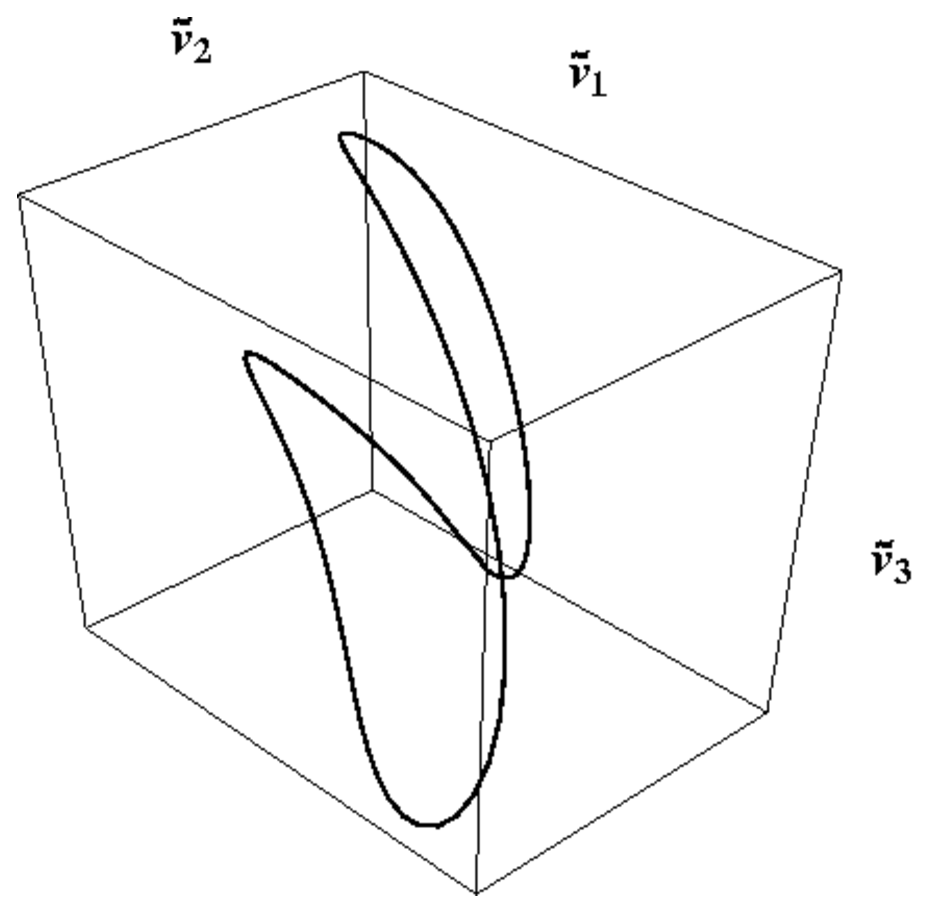
\includegraphics[width=0.40\textwidth, clip=true]
                    {ks22rpo033.50_04.045E2.eps}
~(\textit{b})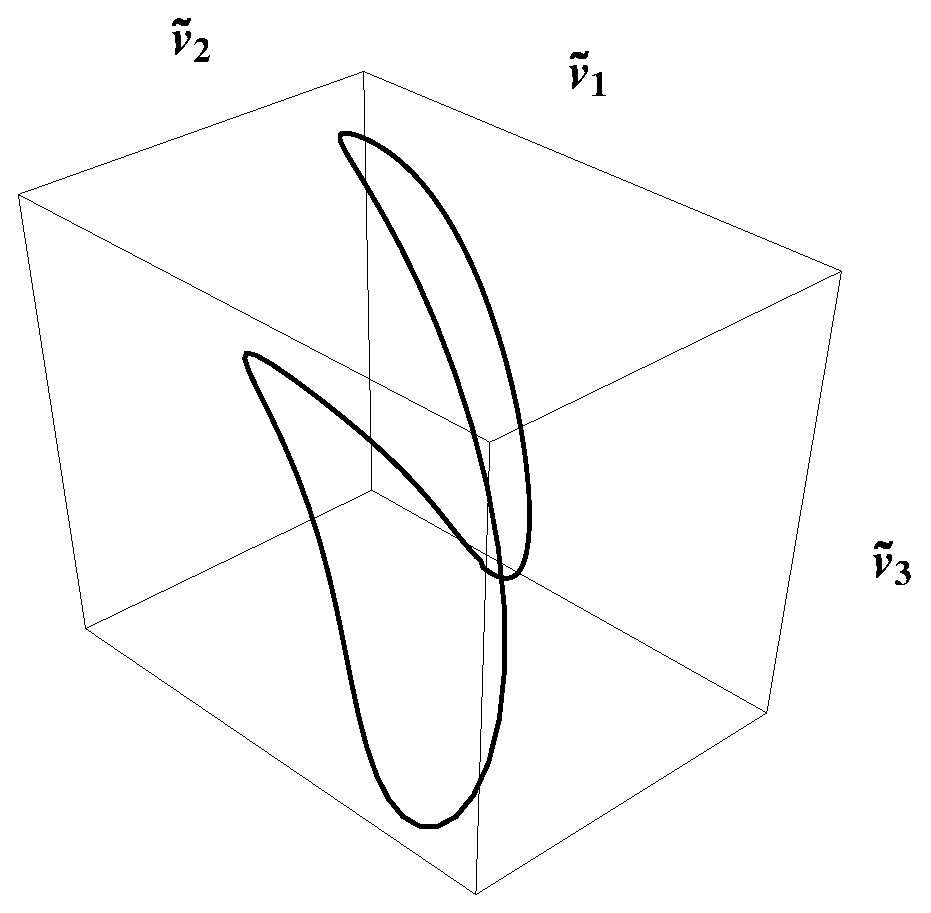
\includegraphics[width=0.40\textwidth, clip=true]
                     {ks22rpo033.50_04.045E2CM.eps}
\caption{
 A \rpo\ of the Kuramoto-Sivashinsky flow, traced for four periods
 $\period{p}$ and projected on
 (a) a stationary \statesp\ coordinate frame
 $\{v_1,v_2,v_3\}$;
 (b) a co-moving $\{\tilde{v}_1,\tilde{v}_2,\tilde{v}_3\}$
 coordinate frame, moving with the mean velocity
 $\velRel_p=\gSpace_p/\period{p}$.
(From \refref{SCD07}.)
}
\end{figure}
%%%%%%%%%%%%%%%%%%%%%%%%%%%%%%%%%%%%%%%%%%%%%%%%%%%%%%%%%%%%%%
%
A \emph{\rpo} is periodic in its mean velocity
$\velRel_p=\gSpace_p/\period{p}$ co-rotating frame,
\reffig{f:MeanVelocityFrame}, but in the stationary frame
its trajectory is quasiperiodic. A co-moving frame is helpful
in visualizing a single `relative' orbit, but useless for
viewing collections of orbits, as each one drifts with its
own group velocity. A simultaneous visualization of all
\rpo s as \po s \JFGedit{can  be attained} only by \emph{symmetry reduction},
to be undertaken in \refsects{s:Hilbert}{sec:mf}.

Relative equilibria and relative periodic solutions are
related to equilibria and periodic solutions of dynamics
reduced by the symmetries. They appear in many physical
situations, such as motion of rigid bodies, gravitational
$N$-body problems, molecules, nonlinear waves, spiralling
patterns and turbulence. According to Cushman,
Bates\rf{CushBat97} and Yoder\rf{Yode88}, C.
Huygens\rf{Huyg1673} understood the \reqva\ of a spherical
pendulum many years before publishing them in 1673. A
reduction of the translation symmetry was obtained by Jacobi
(for a modern, symplectic implementation, see Laskar
\etal\rf{MaRoLa02}). According to Chenciner\rf{Chenc05}, the
first attempt to find (relative) periodic solutions of the
$N$-body problem was the 1896 short note by
Poincar\'e\rf{Poinc1896}, in the context of the 3-body
problem. \Reqva\ of the $N$-body problem (known in this
context as Lagrange points, stationary in the co-rotating
frame) are circular motions in the inertial frame, and {\rpo
s} correspond to quasiperiodic motions in the inertial frame.
\Reqva\ \JFGedit{that} exist in a rotating frame are called central
configurations. For \rpo s in celestial mechanics see also
\refref{Broucke75}. A striking application of \rpo s has been
the discovery of ``choreographies" of $N$-body problems%
\rf{CheMon00,CGMS02,McCordMontaldi}.

The modern story on equivariance and dynamical systems starts
perhaps with M. Field\rf{Field70}, and on bifurcations in
presence of symmetries  with Ruelle\rf{ruell73}. Ruelle
proves that the \stabmat/\jacobianM\ evaluated at an
\eqv/fixed point $\ssp \in \pS_G$ decomposes into linear
irreducible representations of \Group, and that
stable/unstable manifold continuations of its eigenvectors
inherit their symmetry properties, and shows that an \eqv\
can bifurcate to a rotationally invariant periodic orbit
(\ie, \reqv).


\subsection{\label{s:CLEsols} An example: Solutions of \cLe}
% former siminos/CLE/CLEsols.tex

In the case of {\cLe}  the origin \EQV{0} is an \eqv\ of
\refeq{eq:CLe} for any value of the parameters. It is stable
for $0<\RerCLor<\rho_{1c}$ and unstable for
$\rho_{1c}<\RerCLor$, where\rf{FowlerCLE82}
\[
	\rho_{1c} = 1 + {(e+\ImrCLor)(e-\sigma \ImrCLor)}/{(\sigma+1)^2}
\,.
\]
At the bifurcation\rf{ruell73} a pair of eigenvalues crosses
the imaginary axis with imaginary part
\beq
	\omega_c = {\sigma (e + \ImrCLor)}/{(\sigma+1)}
\,,
\ee{eq:omegaCLE}
and a \emph{relative equilibrium} \REQV{}{1} with constant
angular velocity $\omega_c$ is born. For $\omega_c =0$ the
\reqv\ degenerates to an \SOn{2}-orbit of \eqva. As the
existence of a \reqv\ in a system with \SOn{2} symmetry is
the generic situation, we follow \refref{BakasovAbraham93}
and set $\ImrCLor=0$ and $e \neq 0$.

To find the location of the \reqv\ it is convenient to work
\JFGedit{in} polar coordinates
\beq
(x_1,x_2,y_1,y_2,z) =
    (r_1 \cos\theta_1,r_1\sin\theta_1,
     r_2\cos\theta_2,r_2\sin\theta_2,z)
\,,
\label{eq:CartToPol}
\eeq
where $r_1 \geq 0 \,,r_2 \geq 0$.
\JFGedit{The} \CLe\ \refeq{eq:CLe} take \JFGedit{the} form
\[ %\beq
\left(
\begin{array}{c}
\dot{r}_1\\
\dot{\theta}_1\\
\dot{r}_2\\
\dot{\theta}_2\\
\dot{z}
\end{array}
\right)
=
\left(
\begin{array}{c}
 -\sigma\left(r_1 - r_2\cos\theta\right) \\
 -\sigma\frac{r_2}{r_1}\sin \theta  \\
 -r_2 + r_1\left((\rho_1-z)\cos \theta - \rho_2 \sin\theta\right)\\
  e  + \frac{r_1}{r_2}\left((\rho_1-z)\sin\theta +\rho_2 \cos\theta\right)\\
 -b z + r_1 r_2\cos\theta
\end{array}
\right)
,
\] %\ee{eq:PolarCLe}
For
rotationally invariant flows the dynamics depends only
on the relative angle $\theta = \theta_1-\theta_2$
(\JFGedit{which} is why one speaks of `relative' equilibria).
This observation enables us to recast the \cLe\
in the  4-dimensional \reducedsp:
\beq
\left(
\begin{array}{c}
\dot{r}_1\\
\dot{r}_2\\
\dot{\theta}\\
\dot{z}
\end{array}
\right)
=
\left(
\begin{array}{c}
 -\sigma\left(r_1 - r_2\cos\theta\right) \\
 -r_2 + (\rho_1-z)r_1\cos \theta\\
  -e -\left(\sigma\frac{r_2}{r_1}
 +(\rho_1-z)\frac{r_1}{r_2}\right)\sin\theta\\
 -b z + r_1 r_2\cos\theta
\end{array}
\right)
\label{eq:PolarCLeTheta}
\eeq
where we have set $\rho_2=0$. The full 5-dimensional evolution can be
regained by integrating the two driven `reconstruction' equations:
\beq
\left(
\begin{array}{c}
\dot{\theta}_1\\
\dot{\theta}_2
\end{array}
\right)
=
\left(
\begin{array}{c}
-\sigma\frac{r_2}{r_1}\sin\theta  \\
 e + (\rho_1-z)\frac{r_1}{r_2}\sin\theta
\end{array}
\right)
\,.
\label{eq:PolarCLeAngles}
\eeq
In general $\theta_1$ and
$\theta_2$ change in time, but for the \reqva\ the
difference between them is constant.
The condition for a \reqv\ is that all
time derivatives in \refeq{eq:PolarCLeTheta} vanish, while
$\dot{\theta}_1=\dot{\theta}_2\neq 0$ (if
$\dot{\theta}_1=\dot{\theta}_2=0$ we have a group orbit
of \eqva\ instead).
The \reqv\
$\REQV{}{1}$ is given by
\bea
(r_1,r_2,\theta,z) &=&
\left(\sqrt{b \,(\rho_1-d)},  \sqrt{b d \,({\rho_1}-d}),
     \cos^{-1}({1}/{\sqrt{d}}),  \rho_1-d
\right)
\,,
\label{eq:E1-PC}
\eea
where $d=1 + {e^2}/{(\sigma +1)^2}$, and
its angular velocity is
\beq
\dot{\theta}_{i}
= {\sigma e}/{(\sigma + 1)}
\,,
\label{eq:REQV1veloc}
\eeq
with period
$\period{{\REQV{}1}}= 2\pi (\sigma + 1)/\sigma e$.
For the parameter values \refeq{eq:CLeR}, the \reqv\ is at
\beq
\ssp_{\REQV{}1} = (r_1,r_2,\theta,z) =
     (8.48527,
      8.48562,
      0.00909,
      26.9999)
\,,
\label{eq:Q1}
\eeq
rotating with the period $\period{{\REQV{}1}}=69.115$.\ES{Period feels too large,
I'll double check in my notebooks.}

As $\RerCLor$ is increased,  a secondary bifurcation from
\REQV{}{1} results in a \emph{\rpo} \refeq{RPOrelper1}, or,
more precisely, in the quasiperiodic 2-frequency
\emph{modulated traveling wave}\rf{Krupa90}.
Calculation of \JFGedit{the} \REQV{}{1} stability eigenvalues
\PublicPrivate{}{
(see \ref{s:StabReq} for a calculation of stability of
\reqva\ in equivariant variables)
    } %end \PublicPrivate{}{
yields a weakly unstable spiral-out
\eqv\
\beq
(\eigExp_{1,2},\eigExp_3,\eigExp_4)
= (0.0938 \pm 10.1945 i,-11.0009,-13.8534)
\,.
\ee{eq:CLeREQBstab}
With further increase in $\RerCLor$ the dynamics turns
chaotic, with \JFGedit{an} infinity of unstable {\rpo s}. Large numbers of
these can be computed by methods described
elsewhere\rf{SCD07,SiminosThesis}.

The role of \JFGedit{the} above exact invariant solutions is illustrated by the
portrait of \cLf\ \statesp\ in  \reffig{fig:CLE}, with the
\reqv\ \REQV{}{1} and three repetitions of \JFGedit{the} \cycle{01} \rpo\
superimposed over a generic chaotic orbit. Repeats of
\cycle{01} \JFGedit{trace out a torus ergodically} , so in a system with
a $1$-dimensional continuous symmetry the organizational
blocks of a strange attractor are circles (\reqva) instead of
points (\eqva), and partially hyperbolic tori (\rpo s)
instead of closed loops (\po s). It is difficult to
understand the geometry of the flow by looking at such tori.

The large imaginary part of $\eigExp_{1}$ in
\refeq{eq:CLeREQBstab} implies that the simulation has to be
run up to time of order of at least 70 for the strange
attractor in \reffig{fig:CLE} to start filling in. Dynamics
is organized by the interplay of the stable and unstable
manifolds of \eqv\ \EQV{0} and \reqv\ \REQV{}{1}, but the
symmetry-induced drift along the direction of rotation blurs
the picture and the notion of recurrence becomes relative. In
what follows, it is this confusing situation (as well as the
theoretical fact\rf{Cvi07} that dynamical zeta functions have
their support on \rpo s) that motivates the search for
effective methods to project the dynamics onto a \reducedsp.


\section{\label{s:symmRed} Symmetry reduction}
% former siminos/CLE/symRedGeneral.tex

The action of a symmetry group \Group\ on \pS\ endows the
\statesp\ with the structure of a union of group orbits, each
group orbit an equivalence class. The goal of {\em symmetry
reduction} is the identification of a unique point as the
representative of a group orbit, and the replacement of the
original \statesp\ by the space of such points, the {\em
\reducedsp}. In the literature this space is alternatively
called
\emph{desymmetrized \statesp},
\emph{symmetry-reduced space},
\emph{orbit space}, or \emph{quotient space}
$\pS/\Group$ because symmetry has been `divided out.' {The}
symmetry group \Group\ of equivariant dynamics acts trivially
in {the} \reducedsp, and the resulting dynamical system,
called by Gilmore and Lettelier\rf{GL-Gil07b} the
\emph{image}, is symmetry {\em invariant}, in the sense that
its symmetry group is the identity. The mapping {of}
equivariant dynamics to invariant dynamics is implemented by
methods such as
{\em \mframes},
{\em \mslices} or {\em \csection s}, or
{\em Hilbert bases}.

In \refsect{s:Hilbert} we briefly review one of the standard
tools by which spatial symmetry reduction can be achieved:
projection to a Hilbert basis, and show in
\refsect{s:cLeHilbert} how it works for \cLf. A wonderful
symmetry reduction tool for low-dimensional flows, the
Hilbert basis approach turns out to be too cumbersome to be
applicable to high-dimensional flows. Next we describe the
\mframes\ (\refsect{sec:mf}) and apply it to the \cLf\
example to illustrate the form of a general linear slice
(\refsect{sec:CLeMovFr}), show how the \mframes\ enables us
to explicitly compute \Group-invariant coordinates, and
relate these to the Hilbert invariant polynomial basis
(\refsect{s:cleCoordSlice}). Then we discus different choices
of slice-fixing points (\refsect{s:mfReqb}), and the
associated singular sets (\refsect{s:laserMFnum}). Finally,
in \refsect{sec:MovFrameODE}, we recast the essentially
post-processing \mframes\ in the equivalent differential
form, the \mslices, with dynamical equations restricted to
the \reducedsp.


\section{\label{s:Hilbert} Hilbert polynomial bases}

In atomic physics, geophysics and other
low-dimensional physical problems with spatial symmetries,
symmetry reduction is customarily implemented just as we
did it in \refeq{eq:CartToPol}, by going to the `natural'
coordinate system (polar, cylindrical, \etc). That works well
for linear systems, but not so well for nonlinear flows;
note, for example, that these coordinate transformations
introduce non-physical singularities
in \refeq{eq:PolarCLeTheta} at $r_1=0$ and $r_2=0$.

What are we really doing when redefining dynamics in terms of
such invariant coordinates? We are recasting equivariant
dynamics of $(\ssp_1,\ssp_2,\cdots)$ coordinates in terms of
rotationally invariant lengths
$(r_1=(\ssp_1^2+\ssp_2^2)^2,\cdots)$, volumes and other
invariant quantities. Indeed, the problem of symmetry
reduction {was} elegantly solved nearly a century ago.
Physical laws should have the same form in
symmetry-equivalent coordinate frames, so they are often
formulated in terms of functions (Hamiltonians, Lagrangians,
$\cdots$) {that are} invariant under a given set of symmetries. Given a
symmetry, what is the most general functional form of such
law? According to the Hilbert-Weyl theorem, for a compact
group $\Group$ there exists a finite $\Group${-invariant}
Hilbert polynomial basis $\{u_1,u_2, \dots,u_m\}$, $ m \geq
d$, such that any $\Group${-invariant} polynomial can be
written as a multinomial
\beq
h(\ssp) = p(u_1(\ssp),u_2(\ssp), \dots,u_m(\ssp))
    \,,\qquad \ssp \in \pS
\,.
\ee{HilbWeyl}
{The} Gilmore and Lettelier monograph\rf{GL-Gil07b} offers
a very clear, detailed and user friendly discussion of
symmetry reduction by means of Hilbert polynomial bases (do
not look for `Hilbert' in the index, though).
The dynamical equations follow from the chain rule
\beq
 \dot{ u}_i=\frac{\partial u_i}{\partial x_j} \, \dot{x}_j
 \,,
\ee{HilbChainRl}
upon substitution $\{x_1,x_2,\cdots,x_d\}$ $\to$
$\{u_1,u_2,\cdots,u_m\}$. One can either rewrite the dynamics
in this basis, or one can simply plot the `image' of
solutions computed in the original, equivariant basis in
terms of these invariant polynomials.

Unfortunately, while the idea is elegant, an explicit
construction of $\Group${-invariant} basis can in practice be
a laborious undertaking. One trades in the equivariant
\statesp\ coordinates $\{x_1,x_2,\cdots,x_d\}$ for a
non-unique set  of $m \geq d$ invariant polynomials
$\{u_1,u_2,\cdots,u_m\}$. These polynomials are linearly
independent, but functionally dependent through $m - d + N$
nonlinear relations called \emph{syzygies}. Their
determination becomes quickly computationally prohibitive as
the dimension of the system and/or group
increases\rf{gatermannHab,ChossLaut00}, and in practice
typical computations are confined to dimensions less than
ten. As our goal is to quotient continuous symmetries of
high-dimensional flows, high meaning $10^2$-$10^6$ coupled
ODEs, such as those arising from truncations of the \KS\ and
Navier-Stokes flows, {Hilbert basis reduction} is
at present not a feasible option.

Nevertheless, as symmetry reduction of moderate-dimension
flows by the method of invariant polynomials offers a clean
benchmark for other approaches symmetry-reduction, we start
by showing how it works for \cLf.




    \input Hilbert

\section{\label{sec:mf} \Mframes}
    \input movingFrames
    \input mfReqb
    \input mfLocal
    \input slice


\section{Conclusions}
    \input conclusions

\section*{Acknowledgements}
We are grateful to
D.~Barkley,
W.-J.~Beyn,
R.~Gilmore,
J.~Halcrow,
K.A.~Mitchell,
C.W.~Rowley,
R.~Wilczak,
and in particular R.L.~Davidchack for many spirited exchanges,
and J.F.~Gibson for a critical reading of the manuscript.
P.C. thanks the
James Franck Institute, U. of Chicago,
for hospitality, and Argonne National Laboratory and
G.~Robinson Jr. for partial support.
E.S. was supported by NSF grant DMS-0807574 and G.~Robinson,~Jr.

% Specify following sections are appendices. Use \appendix* if there
% only one appendix.
\appendix

\PublicPrivate{}{
\section{\label{s:StabReq} Stability of \reqva}
    \input stabReqva
    } %end \PublicPrivate{}{

% \bibliographystyle{elsarticle-harv}
\bibliographystyle{elsarticle-num}
\bibliography{../bibtex/siminos}

\ifdraft
% remove this when all problems have been fixed
    \newpage
    \input 05fixMe
    \input flotsam
\fi
\end{document}
